\documentclass[oneside,10pt,a4paper,swedish]{scrbook}
\usepackage[T1]{fontenc}
\usepackage[utf8]{inputenc}
\usepackage{babel}
\pagestyle{headings}
\setlength\parskip{1mm}
\setlength\parindent{0pt}
\usepackage{graphicx}
\usepackage{ae}
\usepackage{aecompl}
\usepackage{amssymb}
\usepackage{comment}
%\usepackage{nopageno}
\excludecomment{PROMPT}
\usepackage{bookman}
\usepackage{listings}
\usepackage{float}
\usepackage{multicol}
\setlength\columnsep{4cm}

\usepackage{pxfonts}
\usepackage{geometry}
%\areaset[-1.5cm]{16cm}{26cm}

\newcommand{\tavla}[1]{\reversemarginpar{ \rule[-10mm]{0.1mm}{#1cm}}}


\newcommand{\startex}[1]{\subsubsection{Exempel: #1}}
\newcommand{\slutex}{\vspace{-8mm}\begin{flushright} \rule{1ex}{1ex} \end{flushright}}

\newcommand{\svarsrad}{\begin{flushright} \rule{14cm}{0.2mm} \end{flushright}}
\newcommand{\asm}[1]{\texttt{#1}}

\newcommand{\fth}{\texttt{\textbf{FORTH}}}


\begin{document}

\lstset{basicstyle=\fontsize{10}{3}\selectfont\ttfamily
, tabsize=2}
\title{Datorteknik\\{}BCD-aritmetik\\{}---}

\author{Michael Josefsson}
\date{Version 0.1 2019}

\maketitle
\tableofcontents
\setcounter{chapter}{0}

\chapter{Inledning} Vi har tills nu studerat binära tal med basen två och dess ettor och nollor. En annan talbas som kan vara värd att känna till är den decimala, trots att processorn och logiken fortfarande är binär. 

Med \emph{binärkodade decimala siffror, Binary Coded Digits}, BCD, avses här att de decimala siffrorna \asm{0}--\asm{9} kodas med fyra bitar vardera. Med fyra bitar har vi det hexadecimala talsystemet med sexton symboler \asm{0000}..\asm{1111}. I BCD-fallet används dock bara de som motsvarar de tio symbolerna  \asm{0}--\asm{9}:

\begin{center}
\begin{tabular}{ccc}
Bin & Hex & BCD \\
\asm{0000} & \asm{0} & \asm{0}\\
\asm{0001} & \asm{1} & \asm{1}\\
\asm{0010} & \asm{2} & \asm{2}\\
\asm{0011} & \asm{3} & \asm{3}\\
\asm{0100} & \asm{4} & \asm{4}\\
\asm{0101} & \asm{5} & \asm{5}\\
\asm{0110} & \asm{6} & \asm{6}\\
\asm{0111} & \asm{7} & \asm{7}\\
\asm{1000} & \asm{8} & \asm{8}\\
\asm{1001} & \asm{9} & \asm{9}\\
\asm{1010} & \asm{A} & x\\
\asm{1011} & \asm{B} & x\\
\asm{1100} & \asm{C} & x\\
\asm{1101} & \asm{D} & x\\
\asm{1110} & \asm{E} & x\\
\asm{1111} & \asm{F} & x\\
\end{tabular}
\end{center}

De med 'x' markerade positionerna i BCD-kolumnen är inte tillåtna.

\subparagraph{Omvandling} mellan decimalt tal och BCD sker med tabellen ovan, siffra för siffra.

\startex{Omvandla det decimala talet 6591 till BCD}

\begin{center}
\asm{6591 = 0110 0101 1001 0001 =  0110010110010001}
\end{center}

Den resulterande bitsträngen är i detta fall 16 bitar lång och skulle precis få plats i två byte. Generellt kan en byte husera två BCD-kodade decimala siffror.
\slutex

Man förstår av exemplet att BCD-kodning inte är optimal användning av bitarna, \asm{1010}--\asm{1111} används ju aldrig. Med rent binär tolkning, där alla bitar används, är \asm{6591 = 11001 1011 1111} dvs 13 bitar och 3 bitar kompaktare. Man kanske kan undra varför BCD då blivit en så använd kodning?

Bland fördelarna kan nämnas att utskrifter förenklas avsevärt då talet redan är i presentabel form siffra för siffra. Om det binära talet \asm{1100110111111} skall skrivas ut decimalt måste först de enskilda siffrorna skiljas ut genom en tidsödande ''dela med tio''-process.\footnote{$\frac{6591}{10}=1100110111111/tio=1010010011.0001=659.1$, $1010010011/tio=100001.1001= 65.9$, $1000001/tio=0110.0101=6.5$ och slutligen $0110/tio=.0110=0.6$. Divisionen lämnas som en övning till läsaren.}

Beräkningarna liknar dessutom de vi är vana vid för hand, varför algoritmer är relativt ''rakt på'' att implementera och felsöka.

Precis som vid binära tal kan inte avrundningsfel inträffa vid addition, subtraktion och multiplikation. Av denna anledning är BCD-kodning vanlig i kassaregister där varje öre måste räknas. I detta fall unnar man sig dessutom lyxen att \emph{alltid} använda heltal och placera en decimalpunkt två siffror från höger: \asm{123.45}.

\chapter{Aritmetik} I detta avsnitt beskrivs de grundläggande aritmetiska operationerna addition, subtraktion, multiplikation och division. Läs inte allt på en gång, låt addition sjunka in ordentligt. Allt senare bygger på den.

\section{Addition} Addition av BCD-kodade tal utförs som vanliga decimala tal, med ett viktigt undantag: \textbf{om resultatsiffran efter additionen blivit större än \asm{9} adderas \asm{+6}}. Anledningen till detta inses om man genomför additionen \asm{9} + \asm{1} som med fyra bitar blir hexadecimalt \asm{A}, när det i själva verket skulle bli \asm{0}, dvs man måste vid behov hoppa över de icke tillåtna symbolerna \asm{A}--\asm{F}.

Denna åtgärd kallas decimaljustering, \emph{decimal adjust}, och flera processorer har stöd för BCD-addition inbyggt.\footnote{I Motorola M68000 är stödet inbyggt med instruktioner som \emph{Add BCD} och \emph{Sub BCD}, (\asm{abcd}) och (\asm{sbcd}). I Z80 heter instruktionen \emph{Decimal Adjust Accummulator} (\asm{daa})} 
\startex{Addera 5 + 6 som BCD-kodade tal.}

\begin{center}
\begin{lstlisting}
  5 = 0101
+ 6 = 0110
------------
      1011   = 11, > 9
      0110   + 6 
----c-------
    1 0001   = '11' i BCD
\end{lstlisting}
\end{center}

Additionen gav ett resultat, \asm{1011} som inte är inom det tillåtna området \asm{0}--\asm{9}, varför en ytterligare addition med \asm{+6} genomfördes för att få rätt siffra. Samtidigt noterar man en utgående carry \asm{c} från denna siffra till nästa siffra och resultatet är BCD-mässigt korrekt. 
\slutex

\newpage

Med flera siffror är förfarandet analogt med observationen att man i varje addition kan behöva addera +6. Om den utgående carryn adderas till siffran 9 blir summan \asm{A} och även i detta fall måste addition med +6 utföras. Ett exempel demonstrerar:

\startex{Addera 38 + 75 som BCD-kodade tal.}
För tydlighets skull används här och i fortsättningen ett mellanslag mellan de olika siffrorna. 

\begin{center}
\begin{lstlisting}
  38 = 0011 1000
+ 75 = 0111 0101
----------c------
       1010 1101  = $A respektive $D
       0110 0110    +6 respektive +6
-----c-----------
  0001 0001 0011  = '113' 
\end{lstlisting}
\end{center}
Notera hur en den högra additionen med \asm{+6} gav en carry (\asm{c}) till siffran till vänster.
\slutex

\section{BCD-adderare} På samma sätt som man beskriver addition av binära tal med en fulladderare, FA, kan en full\-adderare för BCD ritas som en komponent som adderar två BCD-siffror plus en inkommande carry och genererar en  BCD-siffra och en utgående carry:

\begin{center}
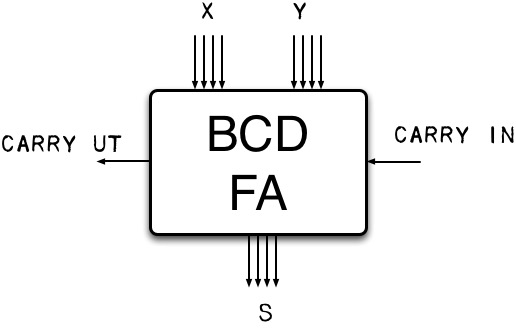
\includegraphics[scale = 0.3]{bcdfa.pdf}
\end{center}

Blocket FA ovan måste alltså innehålla logik som vid behov genomför den önskade extra additionen med \asm{+6}. Addition av flersiffriga tal utförs  med kedjor av fulladderare, en per siffra i talområdet:

\begin{center}
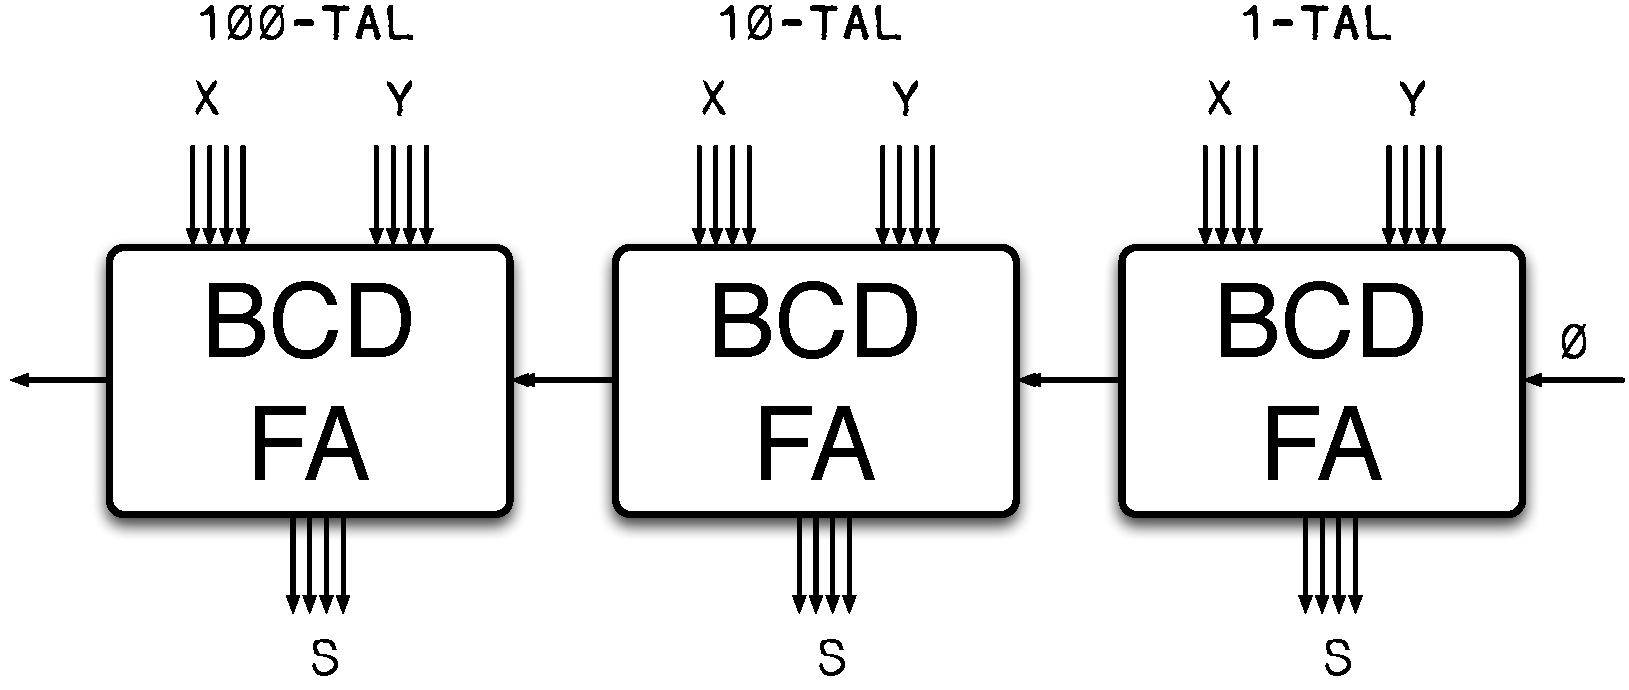
\includegraphics[scale = 0.3]{bcdfas.pdf}
\end{center}


Fulladderarkedjan kan således användas för att addera två åtta-siffriga tal genom att, i en loop, addera talen två och två, och i varje loopvarv $i$ erhålla en carry- och en summabit: \[(C_i,S_i) = X_i + Y_i + c_{i-1} \hspace{5mm}med\hspace{5mm} c_{-1}=0\]

\begin{center}
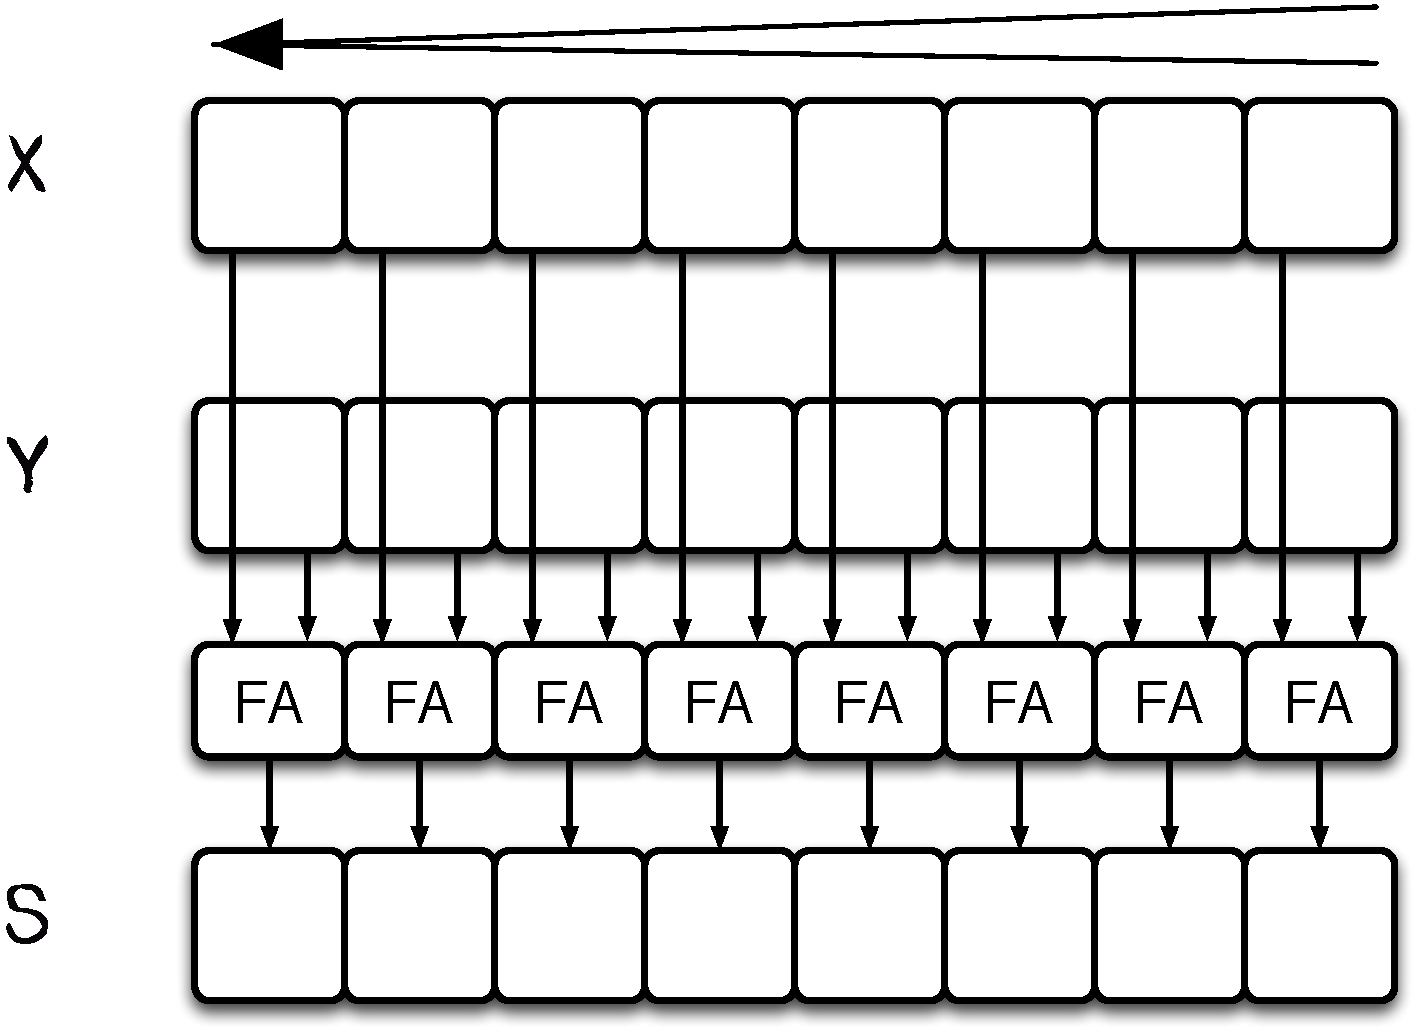
\includegraphics[scale = 0.4]{fakedja.pdf}
\end{center}

I ett program behövs endast en (1) programrutin för fulladderare. Denna rutin underkastas sedan i tur och ordning de ingående talens siffror med början i minst signifikant siffra, från höger till vänster.


\section{Subtraktion} Subtraktion utförs enklast som addition med omvänt tecken. Hittills har talen antagits vara teckenlösa men för subtraktion krävs alltså att vi inför tal med tecken. 

\paragraph{Tio-komplementet} Precis som i tvåkomplementsfallet för basen 2, finns ett \emph{tiokomplement} för basen 10. Genom att komplementera ett tal byts talets tecken. I tvåkomplementsfallet sker detta genom att ett-komplementera (invertera) varje siffra (bit) och addera +1. Tio-komplementering görs på liknande sätt genom att nio-komplementera och addera +1.

I det binära fallet används tvåkomplement och en bit, teckenbiten, indikerar att talet är negativt. I fallet med BCD är situationen något otympligare. Ett ensiffrigt BCD-tal kan med tecken tolkas som:


\begin{center}
\begin{tabular}{r|rrrrrrrrrr|}
 utan tecken    & 0 & 1 & 2 & 3 & 4 & 5 & 6 & 7 & 8 & 9 \\
 \hline
med tecken      & 0 & 1 & 2 & 3 & 4 & --5 & --4 & --3 & --2 & --1 \\
 \end{tabular}
\end{center}

varför alla tal med tecken som inleds med \asm{5}--\asm{9} i själva verket är negativa tal. Det finns alltså inte längre bara en \emph{bit} som anger om talet är negativt.

En konsekvens av detta är att talområdet inte kan vara $\left[-9xxx,\,+9xxx\right]$ utan enbart $\left[-5xxx,\,+4xxx\right]$. För att undvika detta utnyttjas \emph{tecken-beloppsrepresentation} där beloppet, som ju alltid är positivt, blir $\left[0000,\,9999\right]$, och minustecknet hanteras på annat sätt.


Nio-komplementet av en siffra, X, är den siffra som skall läggas till för att summan skall bli 9 enligt nedanstående tabell:

\begin{center}
\begin{tabular}{r|cccccccccc|}
 X    & 0 & 1 & 2 & 3 & 4 & 5 & 6 & 7 & 8 & 9 \\
 \hline
 9--X & 9 & 8 & 7 & 6 & 5 & 4 & 3 & 2 & 1 & 0 \\
 \end{tabular}
\end{center}

\startex{Bestäm BCD-koden för det negativa talet --963.}

Talet är BCD-kodat så att byta tecken på det är detsamma som att tio-komplementera det. Med tabellen ovan, siffra för siffra och en avslutande addition fås


\begin{center}
\begin{lstlisting}
      963   talet
      036   9-komplement
       +1
 ---------
      037   10-komplement
\end{lstlisting}
\end{center}
En kontroll är att \asm{963 + 037 = 1) 000} dvs de tre sista siffrorna adderar ihop till \asm{000}. Den därvid uppkomna carryn kan man bortse ifrån.\footnote{För tre siffror utför man egentligen 1000-komplementet! Och detta genom att beräkna $1000 - x$. Och så vidare.} 


I full BCD-detalj kan komplementeringen utföras som 
\begin{center}
\begin{lstlisting}
      963   1001 0110 0011   talet
      036   0000 0011 0110   9-komplement
       +1   0000 0000 0001  
 ---------
      037   0000 0011 0111  10-komplement
\end{lstlisting}
\end{center}
\slutex

\startex{Ett annat tal, $960$, tio-komplementeras på samma sätt. Glöm inte att decimal\-justera resultatet.}
\begin{center}
\begin{lstlisting}
      960   1001 0110 0000   annat tal
      039   0000 0011 1001   9-komplement
       +1   0000 0000 0001  
 --------------------------
      03A   0000 0011 1010   10-komplement
       +6   0000 0000 0110   DAA
 --------------------------
            0000 0100 0000   10-komplement ('040')
\end{lstlisting}
\end{center}
Som kontroll ser man att $960 + 40 = 10\,000$.
\slutex

\paragraph{Subtraktion}
Med tio-komplementet kan nu subtraktionen $\mathcal{X}-\mathcal{Y}$  utföras som  \[\mathcal{X}-\mathcal{Y}=\mathcal{X}+(-\mathcal{Y})\]

\startex{Utför subtraktionen 2943 -- 698.}
Först tas \asm{-698} fram\ldots
\begin{center}
\begin{lstlisting}
  
    +0698    0000 0110 1001 1000
             1001 0011 0000 0001   9-komplement
       +1    0000 0000 0000 0001   +1
 --------------------------------
    -0698    1001 0011 0000 0010  Koll: 0698 + 9302 = 10000
 
 
 \end{lstlisting}
\end{center}
\ldots och sedan görs en avslutande addition av de två talen:
\begin{center}
\begin{lstlisting}
      2943   0010 1001 0100 0011
   +  9302   1001 0011 0000 0010 
 ---------------c----------------
             1011 1100 0100 0101
         +   0000 0110 0000 0000  Decimaljustera de > 9
 -------------------------------
             1100 0010 0100 0101           
         +   0110 0000 0000 0000  Decimaljustera de > 9
 --------------------------------
             0010 0010 0100 0101  Resultat: +2245
\end{lstlisting}
\end{center}

Här har decimaljusteringen utförts parallellt med alla siffror för att kunna betraktas. Med en ensiffras fulladderare sker denna decimaljustering i varje siffra dock automatiskt.

\slutex


\section{Multiplikation} Multiplikation utförs i huvudsak som upprepad addition men med lite annorlunda disposition än vanligt. En metod anpassad och strömlinjeformad för datorhårdvara blir enklare att implementera än skolmetoden. För enkelhets skull används enbart positiva tal i algoritmen. Den i algoritmerna nedan förekommande additionen utförs i BCD-fallet som komplett addition med decimaljustering.

Först visas multiplikationen på vanligt sätt för att visa de olika del\-resultaten när algoritmen senare anpassas för datorimplementering.

\startex{Multiplicera talen 1234 och 4321.}

Beräkningarna utförs som med decimala tal för att principen bättre skall framgå.

\begin{center}
\begin{lstlisting}
           1234	    multiplikator
           4321     multiplikand
 ---------------
           1234     1234 * 1
          2468      1234 * 2
         3702       1234 * 3
        4936        1234 * 4
 ---------------
        5332114     1234*4321
\end{lstlisting}
\end{center}
\slutex

Algoritmen ovan är känd. Ett problem ur vår synvinkel är att ett antal delresultat måste samlas på hög innan en avslutande, tämligen massiv, addition förlöser det det hela till ett resultat. Det är en nackdel. Men en nackdel som dock kan lösas genom att införa \emph{partialprodukter}, dvs addera så fort något kan adderas. 

\textbf{Not 1.} En multiplikation av två fyra-siffrors tal, en så kallad \emph{4x4}-multiplikation kan inte ge mer än $4+4=8$ siffror i resultatet.

\newpage

Med ledning av detta ansätts en nollställd partialprodukt av önskad längd redan i början:

\subsubsection{Exempel: Partialprodukt}
\begin{center}
\begin{lstlisting}
           1234	     multiplikator
           4321      multiplikand
 ---------------
       00000000      partialprodukt p_0  = 0
           1234      1234 * 1
 ---------------
           1234      partialprodukt p_1       
          2468       1234 * 2
 ---------------
          25914      partialprodukt p_2
         3702        1234 * 3
 ---------------       
         396114      partialprodukt p_3
        4936         1234 * 4
 ---------------
        5332114      partialprodukt p_4 = 1234*4321
\end{lstlisting}
\end{center}
\slutex

Ur denna uppställning och beräkning kan man se hur vissa siffror ändras och hur vissa \emph{aldrig} ändras: I $p_1$ är sista siffran, $4$, redan färdig, klar och beräknad. I $p_2$ tillkommer näst sista siffran, som sedan aldrig ändras, och så vidare. I varje steg tillverkas alltså en ytterligare siffra som  är klar och kan läggas åt sidan. Additionen är i varje steg enbart fyra siffror plus fyra andra siffror! Tyvärr är denna addition mer och mer åt vänster\ldots Men, då det enligt ovan, i varje steg, producerats en siffra till höger kan man skifta partialprodukten ett steg åt höger och på så sätt hålla additionerna rakt under varann.

\subsubsection{Exempel: Partialprodukt och högerskift}
\begin{center}
\begin{lstlisting}
           1234	     multiplikator
           4321      multiplikand
 ---------------
      0000 0000      partialprodukt p_0  = 0
           1234      1234 * 1
 ---------------
      0000 1234      partialprodukt p_1
       000 0123 4    skiftad      
           2468      1234 * 2
 ---------------
       000 2591 4    partialprodukt p_2
        00 0259 14   skiftad
           3702      1234 * 3
 ---------------     
        00 3961 14   partialprodukt p_3
         0 0396 114  skiftad
           4936      1234 * 4
 ---------------
         0 5332 114  partialprodukt p_4 
           0533 2114 skiftad = 1234*4321
\end{lstlisting}
\end{center}
\slutex

\textbf{Not 2.} Generellt erhålls slutresultatet  av en $n\,x\,n$-multiplikation efter $n$ steg. Multiplikationen är i 4x4-fallet alltid i 4 steg.

\textbf{Not 3.} Övre halvan av resultet återfinns under ursprungsoperanderna, undre halvan har producerats under processens gång.

\textbf{Not 4.} För en  $n\,x\,n$-multiplikation behövs enligt ovan endast en $2n$-adderare. Detta gäller generellt.

\paragraph{Multiplikation med tecken} Multiplikationen ovan är beskriven för teckenlösa tal. Med tecken-belopp-representerade tal multipliceras talens belopp och det resulterande tecknet fås genom att betrakta ursprungstalens tecken där olika tecken ger negativt resultat medan samma tecken alltid ger positivt tecken på resultatet.

\paragraph{Multiplikationsdetaljer} I beräkningen ovan utfördes delprodukterna, till exempel \asm{3702 = 1234}$\cdot$\asm{3} utan förklaring. Man kan notera att en sådan delprodukt som mest är en multiplikation mellan ett fyra-siffrigt tal och ett en-siffrigt. Ett enkelt och direkt sätt att utföra denna multiplikation med ett en-siffrigt tal är direkt upprepad addition. Denna sorts ''multiplikation'' tar olika lång tid beroende på antalet additioner men tar under alla förhållanden aldrig mer än högst 9 additioner.

\subparagraph{Fler möjligheter}
\begin{quote}
De ensiffriga multiplikationerna kan beräknas på tre sätt: 

\begin{itemize}
\item upprepade additioner, 
\item tabelluppslagning i en multiplikationstabell eller 
\item använda stöd i befintlig hårdvara.
\end{itemize} 

Metoderna med upprepade additioner eller tabelluppslagning är enklast att implementera. Upprepad addition tar, som nämnts, olika lång tid --- och i bland väldigt lång tid --- beroende på operanderna. Tabelluppslagning tar plats (82 värden) men kan koda hela resultatet i en byte för en total tabellstorlek av 82 bytes. Symmetrier (\asm{3}$\cdot$\asm{4 = 4}$\cdot$\asm{3}) kan användas för att få ner tabellstorleken ytterligare. Inte sällan finns multiplikationsinstruktioner i en processor. I fallet med 8x8-till-16-bitars instruktion kan  denna användas för 1x1-siffras multiplikation (\asm{9}$\cdot$\asm{9 = 81}) enligt ovan, men också för 3x1- eller 2x2-siffrors multiplikation (\asm{999}$\cdot$\asm{9 = 8991}, \asm{99}$\cdot$\asm{99 = 9801}). 
\end{quote}

\newpage

\paragraph{8x8-multiplikation}

Med 8 siffror i både multiplikand och multiplikator blir algoritmen något mer omfattande att visualisera men stegen är desamma:

\startex{Partialprodukt och högerskift 8x8 siffror.}
I detta exempel ansätts plats för maximalt resultat om 16 siffror:
\begin{center}
\begin{lstlisting}
                1736 5289             multiplikator
                3247 5178             multiplikand
 ------------------------
      0000 0000 0000 0000             p_0  = 0
              1 3892 2312             1736 5289 * 8
 ------------------------
              1 3892 2312             p_1
                1389 2231 2           >>
              1 2155 7023             1736 5289 * 7
 ------------------------
              1 3544 9254 2           p_2
                1354 4925 42          >>
                1736 5289             1736 5289 * 1
 ------------------------   
                3091 0214 42          p_3
                 309 1021 442         >>
                8682 6445             1736 5289 * 5
 ------------------------  
                8991 7466 442         p_4
                 899 1746 6442        >>
              1 2155 7023             1736 5289 * 7
 ------------------------  
              1 3054 8769 6442        p_5
                1305 4876 9644 2      >>
                6946 1156             1736 5289 * 4
 ------------------------  
                8251 6032 9644 2      p_6
               	 825 1603 2964 42     >>
                3473 0578             1736 5289 * 2
 ------------------------  
                4298 2181 2964 42     p_7
                 429 8218 1296 442    >>
                5209 5867             1736 5289 * 3
 ------------------------  
                5639 4085 1296 442    p_8             
                0563 9408 5129 6442   >> svar 16 siffror
 ------------------------  
\end{lstlisting}
\end{center}

Den avslutande produkten blir \asm{0563940851296442}. Kontrollera alla siffror på din miniräknare! Om svaret skall ha 8 siffror blir det en användarfråga om det är den första eller sista delen som skall redovisas, eller om ett felmeddelande skall ges ''Svaret får inte plats'' så fort en partialprodukt överstiger 8 siffror.

\slutex


\section{Division}

Division utförs i huvudsak som ''för hand'' med upprepad subtraktion och förflyttning i sidled. Liksom i fallet med multiplikation vill man placera alla subtraktioner och, i förekommande fall, återställande additioner i direkt under varann. 

Först visas divisionen \[\frac{43665}{123} = 355\] enligt  ''liggande stolen'':


\startex{Liggande stolen}
\begin{center}
\begin{lstlisting}
                   123
               _______
           355 | 43665
                -355     1 * 355
                ----
                  816
                 -710    2 * 355     
                -----
                  1065   
                 -1065   3 * 355
                 -----
                     0  
\end{lstlisting}
\end{center}
\slutex

Den inledande subtraktionen är \asm{436}$-$\asm{355} och  går att göra 1 gång innan resultatet blir negativt. Sedan flyttas nämnaren ett steg höger, nästa siffra ur täljaren läggs till och subtraktionen upprepas tills resultatet blir negativt (2 gånger nu) och metoden fortsätter tills alla siffror i täljaren använts.\footnote{Försåvitt inte decimaltal tillåts, ty då fortsätter man på den inslagna vägen, fast  med nollor från täljaren, tills önskat antal decimaler producerats.}

\textbf{Not.} Subtraktionen upprepas tills resultatet är < 0. Den sista subtraktionen återtas och räknas inte in i kvoten.

\newpage

\paragraph{8/8-division}

Metoden går att modifiera med motsvarande knep som i multiplikationsfallet. Utförd i 8 decimala siffror kan den beskrivas enligt nedan där nämnaren är fix i position och storlek medan täljaren flyttas ett steg åt vänster i varje omgång. Nämnaren subtraheras upprepade gånger från täljarens siffror och antalet subtraktioner noteras.


\startex{}
\begin{center}
%\begin{lstlisting}
\begin{lstlisting}
      |00000000|00043665|   startpositioner 
              <<            skift 0
1.    |00000000|0043665-|    
    - |00000355|            0 subtraktioner
      ----------
      |00000000|0043665-| 
              <<            skift 1
2.    |00000000|043665--|   
    - |00000355|            0 subtraktioner
      ----------
      |00000000|043665--| 
              <<            skift 2
3.    |00000000|43665---|    
    - |00000355|            0 subtraktioner
      ----------
      |00000000|43665---|
              <<            skift 3
4.    |00000000|43665---|   
    - |00000355|            0 subtraktioner
      ----------
      |00000000|43665---|    
              <<            skift 4
5.    |00000004|3665----|   
    - |00000355|            0 subtraktioner
      ----------
      |00000004|3665----| 
              <<            skift 5
6.    |00000043|665-----|
    - |00000355|665-----|   0 subtraktioner
      ----------
      |00000043|665-----| 
              <<            skift 6
7.    |00000436|65------|
    - |00000355|            1 * 355 = 81 subtraheras
      ----------
      |00000081|65------|
              <<            skift 7
8.    |00000816|5-------|
    - |00000710|            2 * 355 = 710 subtraheras
      ----------
      |00000106|5-------|
              <<            skift 8, sista
      |00001065|--------|   
    - |00001065|            3 * 355 = 1065 subtraheras
      ----------
              0             rest = 0
\end{lstlisting}
\end{center}
\slutex

Resultatet avläses till höger, uppifrån och ned: 00000123. En 8/8-division tar på detta sätt alltid 8 steg. Det går att snabba upp den genom att studera de ingående talen och vänsterskifta tills första siffran $\neq 0$ finns i entalspositionen men strömlinjeformningen enligt ovan är generell och direkt. Divisionen gick här jämnt ut med resten = 0. I det allmänna fallet ger divisionen dock rest.

\chapter{Implementation}

Medan man mycket väl \emph{skulle} kunna spara BCD-talen som tal med tecken i tio-komplementsform är det sannolikt en onödig komplikation. Den stora fördelen med talen i tecken-belopp-representation är att de alltid är redo att skrivas ut utan behandling. 

Förslagsvis lagras alla resultat i tecken-belopp-representation. Det underlättar felsökning och kontroll av minnesinnehåll då alla tal är direkt avläsningsbara. 

Ett sätt att använda 8 bytes för 8 BCD-siffror är att låta en byte innehålla en BCD-siffra i sin lägsta nibble. Den högsta nibbeln är då fri att använda för att till exempel signalera talets tecken. Det positiva talet 13587195 lagras som

\begin{center}
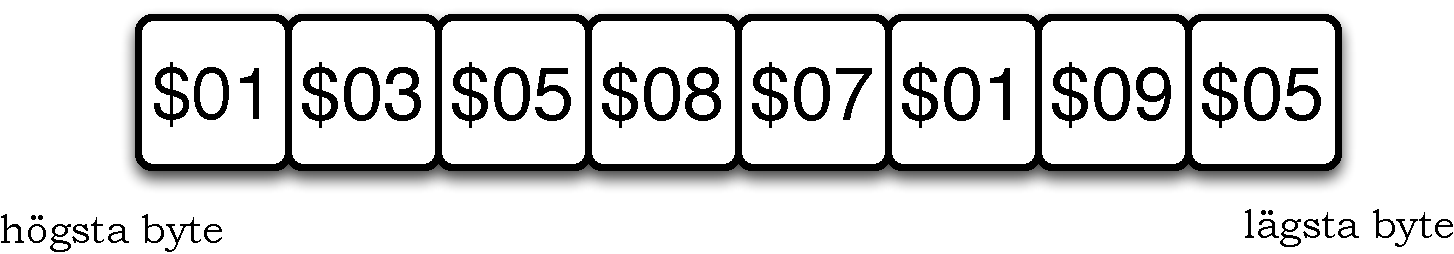
\includegraphics[scale = 0.4]{bcdformat1.pdf}
\end{center}

medan det negativa talet --13587195 lagras med en ''tecken-nibble''

\begin{center}
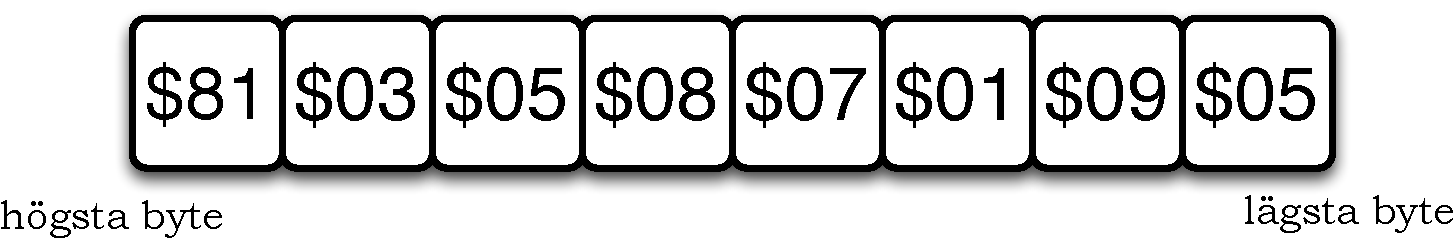
\includegraphics[scale = 0.4]{bcdformat2.pdf}
\end{center}

Med teckenbiten i högsta byten kan utskrift ske genom att först skriva ut ett eventuellt tecken och sedan ignorera alla \asm{\$00}-or tills siffrorna \asm{195} i talet kommer.

En möjlighet är att överföra talet som skall skrivas ut till en intern buffert för utskriftsformattering utan onödiga nollor innan strängen skickas till displayen: \asm{-00001234}$\rightarrow$\asm{-1234}.

\paragraph{Minneslayout}
Som vanligt är en \emph{stack} en lämplig ADT för att lagra numeriska värden för aritmetiska beräkningar. Vill man inte fysiskt flytta runt alla värden på stacken (\asm{push}, \asm{pop} osv) är en stackpekare att föredra. Pekare används sedan hela tiden för att hämta och lagra enskilda siffror vid beräkningarna. 

För enkelhets skull kan man låta alla beräkningar utföras med alla siffror, dvs för att addera två tal måste alla 8 siffror adderas även om talen i sig inte kräver alla 8 positioner.\footnote{Ett litet offer för ökad enkelhet på bekostnad av högsta effektivitet (om högsta effektivitet är  målet använder man inte BCD ändå, right?)}

\begin{center}
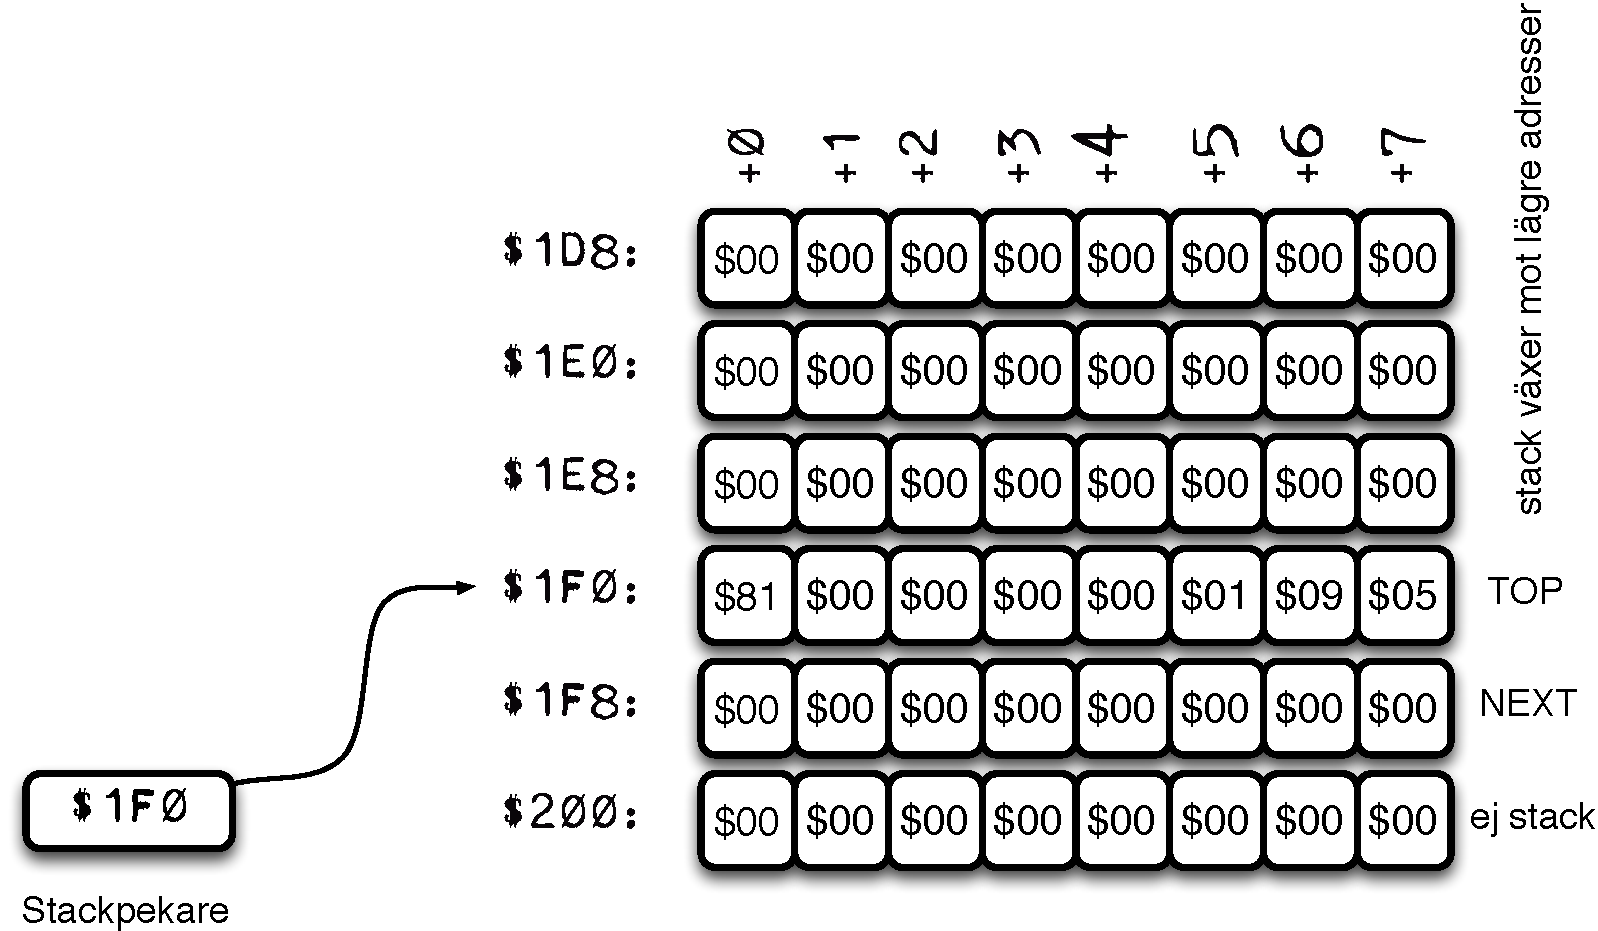
\includegraphics[scale = 0.5]{psp.pdf}
\end{center}

Figuren visar en tänkt minneslayout utförd som en stack där varje tal tar 8 bytes i anspråk. Stackpekaren pekar på  senast ditlagda tal, här talet --195 respektive 0. Med en bestämd maximal tallängd om 8 bytes är upp/ned-räkningen till nästa/föregående tal alltid samma.\footnote{Faktum är att de tre lägsta bitarna i adressen är respektive byte-adress inom ett tal.} 

Fördelen är att stacken enkelt kan manipuleras med rutiner som \asm{drop} och \asm{dup} men även med mer komplexa rutiner som \asm{+}, \asm{-} och \asm{negate} med flera.\footnote{Lägg märke till att en subtraktion utförs som ''call negate, call plus'' om en paraeterstack används.} Ett tal behöver aldrig \emph{raderas} från stacken, ej heller nollställas, det räcker att peka om stackpekaren. I figuren ovan innehåller de inte utnyttjade talen enbart \asm{\$00}, detta är inte nödvändigt och i verkligheten osannolikt.

En ytterligare fördel är att stacken även kan används \emph{internt} i respektive aritmetisk beräkning för att lagra mellanresultat! Genom att nå respektive siffra i talen med pekare kan effektiva programflöden uppnås.

\appendix
\chapter{8x8-multiplikation med upprepad addition}
Här visas multiplikationen \asm{1234}$\cdot$\asm{4321} med upprepad addition utskriven i varje steg.
\startex{Partialprodukt och högerskift, alla steg}
\begin{center}
\begin{lstlisting}
           1234	     multiplikator
           4321      multiplikand
 ---------------
      0000 0000      partialprodukt p_0  = 0
           1234      1234 * 1
 ---------------
      0000 1234      partialprodukt p_1
            123 4    skiftad      
           1234      1234 * 2
           1234      
 ---------------
      0000 2591 4    partialprodukt p_2
            259 14   skiftad
           1234      1234 * 3
           1234
           1234
 ---------------     
      0000 3961 14   partialprodukt p_3
            396 114  skiftad
           1234      1234 * 4
           1234
           1234
           1234
 ---------------
      0000 5332 114  partialprodukt p_4 
           0533 2114 skiftad = 1234*4321
\end{lstlisting}
\end{center}
\slutex

\chapter{\emph{Double dabble}-algoritmen}

Ibland kan befintlig hårdvara för binär multiplikation användas. För att använda sådana basen-2-resultat i decimalaritmetiken måste de först omvandlas till BCD-tal.

För omvandling mellan binära tal och BCD-tal kan en variant av den s.k. \emph{double dabble}-metoden användas. I grova drag utförs successiva vänsterskiftningar av det binära talet och siffran 6 adderas\footnote{I en vanlig implementation av metoden utförs istället addition med 3 innan vänsterskiftningen.} om resultatet i en BCD-kolumn (här ''10'' och ''1'') blir större än 9:

\startex{Omvandla \asm{1100}$_2$ till BCD med \emph{double dabble}-algoritmen}
\begin{center}
\begin{tabular}{c|c|c|l}
Op & 10 & 1 & Binär-tal\\
\hline
Start & \asm{0000} & \asm{0000}&\asm{1100}\\
Skift & \asm{0000} & \asm{0001}&\asm{100}\\
Skift & \asm{0000} & \asm{0011}&\asm{00}\\
Skift & \asm{0000} & \asm{0110}&\asm{0}\\
Skift & \asm{0000} & \asm{1100}&$\leftarrow$ större än 9\\
6	  & \asm{0000} & \asm{0110}&$\leftarrow$ addera 6\\
+     & \asm{0001} & \asm{0010}&\asm{}\\
\hline
BCD & \asm{1} & \asm{2}&$\leftarrow$ svar i BCD\\
\end{tabular}
\end{center}

Med resultatet i BCD-form kan det användas för att adderas till partialprodukten i den ursprungliga multiplikationen.

\begin{center}---o=Ö=o---\end{center}
\end{document}
